%\svnInfo $Id: Ch1_2017.tex 65 2017-08-14 19:39:16Z Georg Lindgren $ 
%$
%
%=========
\chapter{Introduction to \progname{}}\label{cha:introduction}\label{cha:1}
%=========

\section{What is WAFO?}\label{sec:whatiswafo}
\progname{} (Wave Analysis for Fatigue and Oceanography) is a toolbox of
Matlab routines for statistical analysis and simulation of {\em random
waves} and {\em random loads}. Using {\sc Wafo} you can, for example,
calculate theoretical distributions of wave characteristics from
observed or theoretical power spectra of the sea or find the
theoretical density of rainflow cycles from parameters of random loads. 
These are just two examples of the variety of problems you can analyze
using this toolbox.

There are three major audiences to which this toolbox can have a great
deal of appeal. First, {\em ocean engineers} will find a comprehensive
set of computational tools for statistical analysis of random waves and
ship's responses to them. Second, the toolbox contains a number of
procedures of prime importance for {\em mechanical engineers}
working on {\em random loads} or {\em damage and
fatigue analysis}.  Finally, any {\em researcher} who is interested in
{\em statistical analysis of random processes} will find an
extensive and up-to-date set of computational and graphical tools, 
including simulation from spectrum of Gaussian and non-Gaussian 
processes and fields. 

In a random wave model, like that for Gaussian or transformed
Gaussian waves, the distribution of wave characteristics such as wave
period and crest-trough wave height can be calculated with high
accuracy for almost any spectral type. {\sc Wafo} is a third-generation
package of \ML{} routines for handling statistical modelling,
calculation and analysis of random waves and wave characteristics and
their statistical distributions. The package also contains routines
for cycle counting and computation in random load models, in
particular the rainflow counting procedure often used in fatigue life
prediction.

Random wave distributions are notoriously difficult to obtain in
explicit form from a random wave model. 
However, numerical algorithms,
based on the so-called regression approximation and on contemporary 
methods to compute very high-dimensional normal integrals, work very well 
and are simple to use with context specific interface, included in \wf{}. 
These
methods to calculate wave distributions are the only known methods that
give correct answers valid for general spectra. The theoretical
background is reviewed in \cite{LindgrenAndRychlik1991Slepian}
% LiRy91 %Lindgren and Rychlik (1991)
and computational aspects and algorithms in
\cite{RychlikAndLindgren1993Crossreg} and 
\cite{Brodtkorb2006Evaluating,PodgorskiEtal2000Exact}. 
%RyL93}. %Rychlik and Lindgren (1993).

The algorithms are based on a specification of the random waves by
means of their (uni-directional or directional) spectrum, and on the
underlying assumption of linear wave theory and Gaussian
distribution. For non-Gaussian waves, \wf{} offers three alternatives. 
The first is simple though often sufficient, is to use a transformation 
of sea elevation data to obtain a 
desired (horizontal) asymmetric marginal distribution. 
The two others include second order wave theory, and a Langrange 
horizontal transformation of the wave field, respectively. 

A first complete toolbox appeared
1993, called the Fatigue Analysis Toolbox (FAT)\index[xentr]{FAT},
\cite{FrendahlEtal1993Fatigue}.
It was followed by the
Wave Analysis Toolbox
(WAT\footnote{\url{http://www.maths.lth.se/matstat/staff/georg/watinfo.html}
})\index[xentr]{WAT} in 1995, written by Rychlik and Lindgren,
\cite{RychlikAndLindgren1995Wave},
being extended with routines for probabilistic modelling problems in
oceanography. In {\sc Wafo}, presented 2000, \cite{BrodtkorbEtal2000Wafo}, 
a considerable improvement in computational speed and accuracy was achieved. 
Many new routines were introduced, for example routines for spatial waves 
with time dynamics, thus extending the analysis to random fields. Algorithms for
rainflow analysis of switching Markov chains as well as 
for decomposition of the rainflow matrix were included.
 Many of the new tools were the result of new research, e.g.\
\cite{RychlikEtal1997Modelling,PodgorskiEtal2000How,
PodgorskiEtal2000Exact,Johannesson1999Rainflow,BrodtkorbEtal2001Joint}.

\progname{} version 2.5 appeared in beta-version January 2009,
and in stable version February 2011, adding a great
number of general statistical routines, making the toolbox useful
also for statistical analysis in many other areas than
marine and mechanical engineering; see \verb+help statistics+. 
In 2016, routines for simulation and analysis 
of non-Gaussian Lagrange waves were added. The present version 
of the toolbox  simply called \progname{} with year 2017 to indicate 
tested \ML{} version.

From version 2.5, \progname{} has a modular structure, 
so users can easily add their
own algorithms for special purposes. The modules of the toolbox handle
\begin{itemize}\setlength\itemsep{-1mm}
  \item wave/load data analysis and estimation,
  \item spectral distributions,
  \item transformation to Gaussian marginals and calculation of
exact distributions,
  \item simple parametric approximations to wave
        characteristic distributions,
  \item simulation of Gaussian and Markovian wave/load time series,
  \item simulation of Lagrange wave fields and second order models, 
  \item extreme value and other statistical analysis,
  \item cycle counting,
  \item rainflow cycle analysis and calculation,
  \item fatigue life calculation,
  \item smoothing and visualization,
  \item general statistical analysis and computation.
\end{itemize}

In the following section, we discuss in more detail the idea
of the modular structure. That section is followed by an overview of
the organization of \progname{}, presenting some of the capabilities of the
toolbox. Finally, we give a number of examples to demonstrate the use
of some of the tools in \progname{} for analysis and modelling.

%=========================================
\section{Philosophy -- some features of \progname{}}\label{sec:philosophy}
%=========================================

A common problem with research involving complex scientific (numerical)
computations is that when researchers try to advance and leverage their
colleagues work, they often spend a considerable amount of time just
reproducing it.

Often after few months since the completion of their own work, authors
are not capable of reproducing it without a great deal of agony, due to
various circumstances such as the loss of the original input data
or/and parameter values etc.  Thus many scientific articles are
reproducible in principle, but not in practice.

To deal with this and to organize computational scientific research and
hence to conveniently transfer our technology, we impose a simple filing
discipline on the authors contributing to the \progname{}-toolbox.
(A positive side effect of this discipline is a reduced amount of
errors which are prone to occur in computational science.)

This philosophy was inspired by the article by Matthias Schwab et
al~``Making scientific computations reproducible'', 
\cite{Schwab:2000:MSC:369545.369555}. 
The idea is to develop reproducible knowledge about the results of the
computational experiments (research) done and to
make it available to other researchers for their inspection,
modification, re-use and criticism.

As a consequence, \progname{} is freely available through the
Internet\footnote{\url{https://github.com/wafo-project}}.  
Other
researchers can  obtain  the \ML{} code that generated figures in
articles and reproduce them.  They can if they wish modify the
calculations by editing the underlying code, input arguments and
parameter values.  They can use the algorithms on other data sets or
they can try their own methods on the same data sets and compare the
methods in a fast and easy fashion.

This is the reason of existence for the \verb+WAFO/papers+ directory,
which contains subdirectories including scripts for recreating figures
in published articles and technical reports.  Each article has its own
subdirectory.  The directories contain demonstration scripts to
generate individual figures and (possibly) specialized tools/functions
not available in the official release of \progname{} for generating these
figures.

Just like the \verb+WAFO/papers+ directory, the \verb+WAFO/wdemos+ directory
also contains different
subdirectories with scripts producing figures.  The only difference is that
these do not reproduce figures from published articles but merely test and
demonstrate various methodologies, highlight some features of \progname{},
and release code that approximately
reproduces figures in other articles.
The important thing for both directories is not the printed figures,
but the underlying algorithm and code.
In addition, the \verb+papers+ and \verb+wdemos+ scripts constitute
an excellent starting point for the novel user to learn about \progname{}.

The documentation directory \verb+WAFO/docs+ contains 
documentation available for the toolbox, mostly as PDF-files. 
% The contents of any of these files may be examined by typing 
%its name for ascii files or viewing in ghostview for postscript files.
Also each function is well documented containing a help header
 describing how the function works with a detailed list of
input and output arguments with examples of how to use the function.

The Matlab code to each function file also contains references to
related functions and  reference to published
articles from which the user can obtain further information if such exist.

One important element in the toolbox is the use of
\textsl{structure arrays}, introduced in \ML{}, Version 5, by which
several types of data can be stored as one object.
This significantly simplifies the passing of input and output arguments
of functions and also makes the \ML{} workspace much tidier when working
with the new toolbox compared to the old ones.
Three general data structures or object classes are implemented and
extensively used: spectrum structure, covariance structure, and
probability density function (hereafter denoted pdf) structure. 
Other structures are used, e.g.\ to set parameters for numerical computation and  
simulation 

The most complete implementation of the \wf{} toolbox is  the 
one for Windows~10, working together with \ML{}. A reduced set can be 
used with Linux platform together with {\sc Octave}. 
%The toolbox is portable to any
%computational environment that supports \ML{}, such as Linux, Unix or
%PC with MS Windows. See Section~\ref{sec:datastructures} for a description
%of the datastructures in {\sc Wafo}{}. Note that this tutorial
%uses the command naming convention introduced in \progname{}, Version 2.5.



All the files in the package are located in subdirectories under the main
directory. The following directories are related to what has been
discussed above. In the next section, we describe in more details the
directories (or modules) which contain routines for application.
\begin{description}\setlength\itemsep{-1mm}
\item[] \verb+WAFO+ is the main directory containing different directories for the
  \progname{} software, datasets and documentation.
\item[] \verb+WAFO/docs+ contains the documentation for the toolbox.
\item[] \verb+WAFO/papers+ is a subdirectory including scripts for reproducing
  figures in various articles and technical reports. The scripts {\tt tutorcom} 
  for the examples in this tutorial are found here.
\item[] \verb+WAFO/wdemos+ contains different demonstrations that illustrate and
  highlight certain aspects of \progname{}.
\item[] \verb+WAFO/data+ contains datasets used in the demo and paper scripts.
\item[] \verb+WAFO/source+ contains {\tt mex} and {\sc Fortran} source files.
\item[] \verb+WAFO/exec/...+ contains {\sc Fortran} compiled executables for different
  platforms and \ML{} versions.
\end{description}

%===========================================
\section{Organization of \progname{}}\label{sec:WAFOorganization} %

In this section, we make a brief presentation of each module.
%The text will not be a complete list of routines; such
%a list may be found at the web site for \progname{}. 
We want to emphasize
that all routines in \progname{} work together -- the division into
sub-toolboxes is only to make it easier for the user to find the routines
for the actual problem.
%\vspace*{-3mm}

\subsubsection{Data analysis}
Routines in the category {\tt onedim} treat data in the form of time series.
As examples of routines, we find procedures for extraction of
so-called turning points, from which troughs and crests may be obtained,
as well as procedures for estimation of auto-covariance function and
one-sided spectral density. One routine extracts wave heights and
steepnesses. Numerous plotting routines are included. 

Routines in the category {\tt multidim} treat multidimensional problems in 
space and time. One routine estimates a directional spectrum from a 
series of wave field measurements, and other routines handle 
problems with directional spreading and wave measurements. 

\subsubsection{Spectrum}
Computation of spectral moments and covariance
functions, given a spectrum, is a necessary step for
calculation of exact probability distributions of wave
characteristics. The spectrum structure mentioned in the
previous section allows this calculation to be performed for
directional spectra as well as encountered spectra.
We present routines for calculations of commonly used frequency
spectra $S(\omega)$, e.g.~{\sc Jonswap} and Torsethaugen. The spectra can be
expressed in frequency as well as wave number. Libraries of
spreading functions $D(\theta)$, in some cases allowed to be
also frequency dependent, cf. \cite{KrogstadAndBarstow1999Directional},
%{KB9}, %~Krogstad and Barstow (1999),
are included.%\vspace*{-3mm}

\subsubsection{Gaussian and related processes -- exact results}
A unique feature of the \wf{} toolbox is its capacity to deliver the
exact statistical distribution of wave characteristics of linear, Gaussian waves, 
given a spectrum; for example
\begin{itemize}\setlength\itemsep{-1mm}
    \item pdf for apparent wavelength and period,
    \item joint pdf for wavelength (period) and amplitude,
    \item joint pdf of half wavelengths.
\end{itemize}
Routines for transformed Gaussian processes, cf.\
\cite{RychlikEtal1997Modelling}, %RyLJ97}, % Rychlik et.~al (1997),
are included. Contrary to what is often stated in the technical literature,
these routines are very efficient and accurate and they can be used for
engineering purposes; cf.\ \cite[Sec.\ 4.4.1]{Massel1996Ocean}. %\vspace*{-3mm}

\subsubsection{Simulation of random processes and fields}
Efficient simulation of a Gaussian or transformed Gaussian process $X(t)$ and its
derivative $X'(t)$, given the spectral density or the
auto-correlation function, can be performed. 
For fast and exact simulation, some routines use
a technique with circulant embedding of the covariance matrix,
\cite{DietrichAndNewsam1997Fast}. %,DN97}. %       Dietrich and Newsam (1997).
More traditional spectral simulation methods (FFT) are also used. 
Space-time simulation of non-linear wave fields can be made to generate front/back and 
crest/trough asymmetric 3D waves, including second order Stokes waves and 
Lagrange waves with directional spreading. 

Simulation of discrete Markov
chains, Markov chains of turning points, switching Markov
chains and Hidden Markov Models, etc, is possible.
Other routines generate time-varying random (Gaussian or transformed
Gaussian) wave fields with directional spectrum.
%\vspace*{-3mm}

\subsubsection{Parametric wave models}
In \progname{}, we have implemented cer\-tain models for distributions
of wave characteristics found in the literature. For example,
one finds
\begin{itemize}\setlength\itemsep{-1mm}
   \item approximations of the density of crest period and amplitude,
     $(T_c,A_c)$, in a
   stationary Gaussian transformed process proposed in
   \cite{CavanieEtal1976Statistical},
 %,CAE76}, %(Cavani\'e, Arhan and Ezraty (1976),
   and \cite{Longuet-Higgins1983Joint},%LH83}, % (1983))
   \item a model for the cdf/pdf of breaking limited wave
   heights proposed in \cite{Tayfun1981Breaking},%Tayfun81}, %(Tayfun (1981))
   \item a model for the cdf/pdf of large wave heights
   in \cite{Tayfun1990Distribution}.%Tayfun90}. %(Tayfun (1990))
\end{itemize}
These are parametric models, where the calculations need as input the spectral 
moments, as opposed to the algorithms in the
exact Gaussian module, where the whole spectrum is required. %\vspace*{-3mm}

\subsubsection{Discretization and cycle counting}
After extraction of the so-called sequence of turning points
(the sequence of local maxima and minima) from data, cycle
counts can be obtained, e.g.~max-to-min cycles, trough-to-crest cycles,
rainflow cycles. For descriptive statistics, the counting
distribution and the rainflow matrix are important; these can
be obtained. Given a cycle matrix, one can obtain histograms for
amplitude and range, respectively. %\vspace*{-3mm}

\subsubsection{Markov models}
If the sequence of turning points forms a Markov chain it
is called an MC of turning points (MCTP).
The Markov matrix is the expected histogram matrix of min-to-max
and max-to-min cycles. Given a rainflow matrix of an MCTP, one can
find its Markov matrix, and vice versa.
In \progname{}, algorithms are implemented to
calculate the rainflow matrix for an MC and an MCTP;
cf.\ \cite{FrendahlAndRychlik1993Rainflow}.
%,FrRy93}. % cf.~Frendahl and Rychlik (1993).

In some applications, one wants to model data, whose properties
change according to an underlying, often unobserved process,
called the regime process. The state of the regime process
controls which parameters to use and when to switch the
parameter values. If the regime process is modelled by a
Markov chain we have a Hidden Markov Model (HMM),
and this is the fundamental basis for the set of
routines presented. For an application with such switching Markov
models for fatigue problems,
see \cite{Johannesson1998Rainflow,Johannesson1999Rainflow}.%Jo98,Jo99}.
%\vspace*{-3mm}% cf.~Johannesson (1998), (1999).

\subsubsection{Fatigue and Damage}
In \progname{}, routines for calculation of the accumulated damage
according to the Palmgren-Miner rule have been implemented. It
is possible to compute the total damage from a cycle count as
well as from a cycle matrix. The relation between load energy spectrum 
and fatigue can be analysed by using the spectrum 
for a transformed Gaussian load process to first calculate a cycle matrix 
and then the total damage. See {\tt help fatigue} for a list of 
fatigue routines 
available in the different \wf{} directories. %\vspace*{-3mm}

\subsubsection{Extreme value distributions}
Certain probability distributions are extensively used in
ocean engineering, e.g. Rayleigh, Gumbel, Weibull. The
generalized extreme-value distributions (GEV) and generalized
Pareto distributions (GPD) are also important. For these and other
popular distributions, used in reliability and
life-span models, it is possible to estimate parameters,
generate random variables, evaluate pdf and cumulative
distribution function, and plot in
various probability papers.
% One category of routines handles
% bivariate distributions. Besides having routines for estimation
% of parameters etc.~for the two-dimensional Weibull distribution,
% bivariate modelling is possible.
%\vspace*{-2mm}

\subsubsection{Kernel-density-estimation tools}
The routines in this category complement the ones found in
'Data analysis' and, obviously, the routines in
'Statistical tools and extreme value distributions'.
They are, however, also applicable to multi-dimensional data,
and hence very useful for smoothing purposes when comparing
(theoretical) joint distributions of wave characteristics to
data;
cf.\ \cite{Silverman1986Density} and %Si86}, % cf.~Silverman (1986),
\cite{WandAndJones1995Kernel}.%,WJ95}.
%\vspace*{-3mm} % Wand and Jones (1995).

\subsubsection{\progname{} as a statistics toolbox}
Besides the special statistical routines for extreme value analysis
and kernel smoothing,  \progname{} contains statistical routines for
handling univariate and multi-variate distribution functions,
simulation, moments, likelihood estimation, regression and factor
analysis, hypothesis testing and confidence intervals, bootstrap and
jackknife estimation, and design of experiment.

\subsubsection{Miscellaneous routines}
We find here various plot routines, algorithms for numerical
integration, and functions for documentation of \progname{} with
modules. Note, that the figures in this tutorial have been edited with
respect to font size, and some other properties.

%==============================================
\section{Some applications of \progname{}}\label{sec:WAFOapplications}
%==============================================
In this section we demonstrate some of the
capabilities of \progname{}. For further examples and knowledge about the
algorithms used in the routines, we refer to the tutorial and the
documentation in the routines. The necessary \ML{} code
for generation of the figures in this tutorial is found in the directory
\verb+WAFO/papers/tutorcom/+. The commands for this chapter are collected in
\verb+Chapter1.m+ and run with \ML{ 9.1} in 5 seconds on a 3.6~GHz 64 bit PC with Windows 10.

  %-----
\begin{figure}
  \centering
  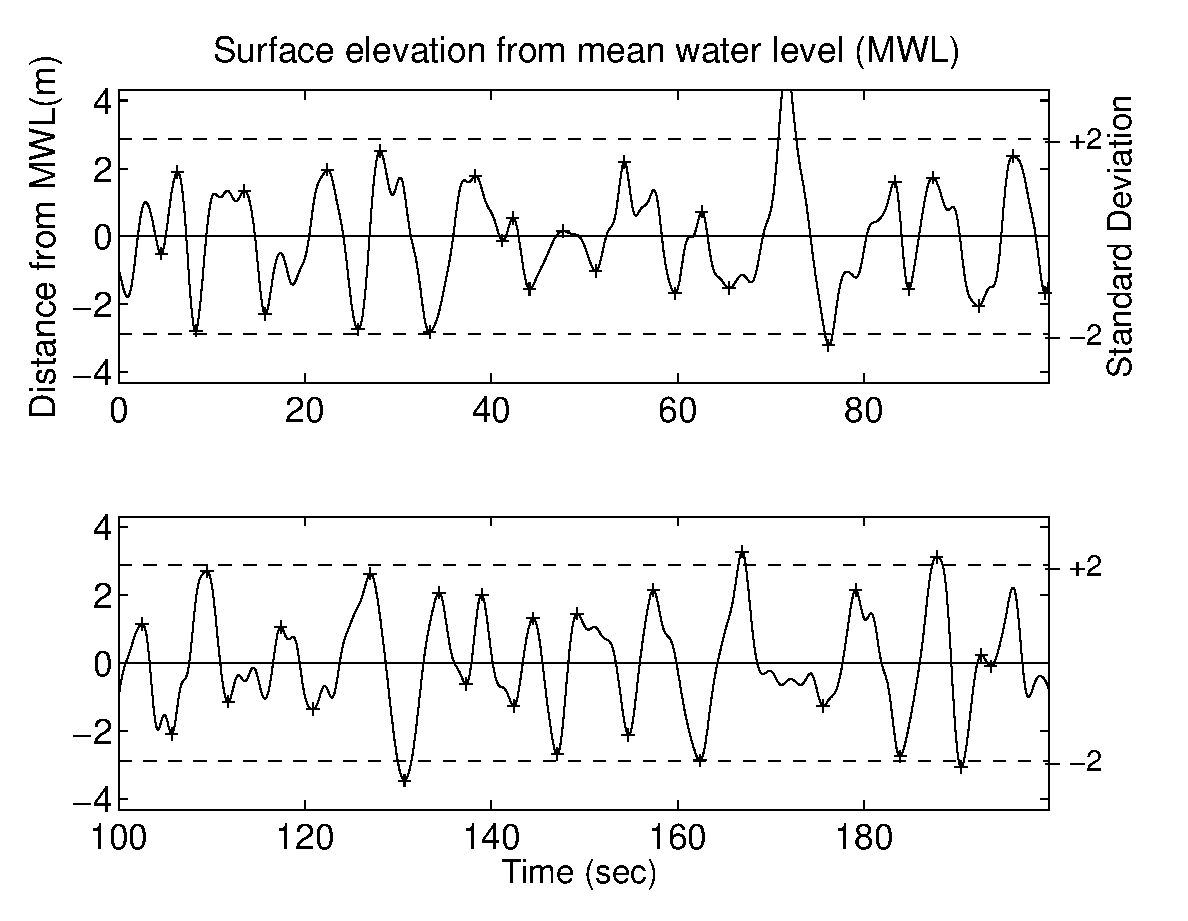
\includegraphics[width=\onefigwidth]{001f_sim}
%\psfig{figure=./Nyabilder/001f_sim.eps,width=\onefigwidth}
\vspace{-3mm}
\caption[Example of simulated wave profile]{A simulation
    from $S(\omega)$, a Torsethaugen spectrum with
    $H_{m_0}=6$~[m], $T_p=8$~[s].  Total number of points
    $=2000$, $\Delta t=0.1$~[s].}
\label{fig:simulation}
\end{figure}
  %-----

  We start by defining a frequency spectrum, $S(\omega)$, which will be
  used in many of the examples; we choose a Torsethaugen spectrum with
  the parameters $H_{m_0}=6$ [m], $T_p=8$ [s], describing significant wave
  height and primary peak period, respectively. The energy is divided
  between two peaks, corresponding to contributions from wind and swell;
  \cite{Torsethaugen1996Model}. % Torsethaugen 1996).
  \progname{} allows spectra to be defined simply by
  their parameters $H_{m_0}$ and $T_p$. The list in Section~\ref{s:ListOfSpectra} 
  helps to keep track of the different theoretical and empirical spectra we use in this tutorial. 
  \index[xentr]{spectrum!list of spectra used}

  %==============================================
  \subsection{Simulation from spectrum, estimation of spectrum}%---
  %==============================================
\index[xentr]{simulation!from spectrum}

  In Figure~\ref{fig:simulation}, plotted using {\tt waveplot},
  we have simulated a sample path from
  $S(\omega)$. \index[xcmds]{{\tt waveplot}}
 %The algorithm can equally well have the covariance function as input.
  The user specifies the number of wanted points in
  the simulation.  The following code in  \ML{}
  generates 200 seconds of data sampled with 10 Hz
  from the discussed spectrum. More on simulation can be found in
  Section~\ref{sec:simulationofGaussian}. \index[xcmds]{{\tt plotflag}}
{\small\begin{verbatim}
      Hm0 = 6; Tp = 8; plotflag = 1; clf
      ST = torsethaugen([],[Hm0 Tp],plotflag);
      dt = 0.1; N = 2000;
      xs = spec2sdat(ST,N,dt); clf
      waveplot(xs,'-')
\end{verbatim}}\index[xcmds]{{\tt spec2sdat}}

In a  common situation, data is given in form of a time
series, for which one wants to estimate the related spectrum.
We will now simulate 20 minutes of the signal sampled with 4~Hz,
find an estimate $S_{\mbox{\footnotesize est}}(\omega)$ and compare the
result to the original Torsethaugen spectrum $S(\omega)$.
The following code was used to generate Figure~\ref{fig:spectra},
where the original and estimated spectra are displayed. The maximum
lag size of the Parzen window function used (here 400) can be chosen
by the user or automatically by \progname{}. \index[xentr]{window!Parzen}
{\small\begin{verbatim}
      plotflag = 1; Fs = 4; clf
      dt = 1/Fs; N  = fix(20*60*Fs);
      xs = spec2sdat(ST,N,dt);
      STest = dat2spec(xs,400)
      plotspec(ST,plotflag), hold on
      plotspec(STest,plotflag,'--')
      axis([0 3 0 5]), hold off
\end{verbatim}}

    \index[xcmds]{{\tt plotspec}}

  %-----
  \begin{figure}[tbh]
    \centering
    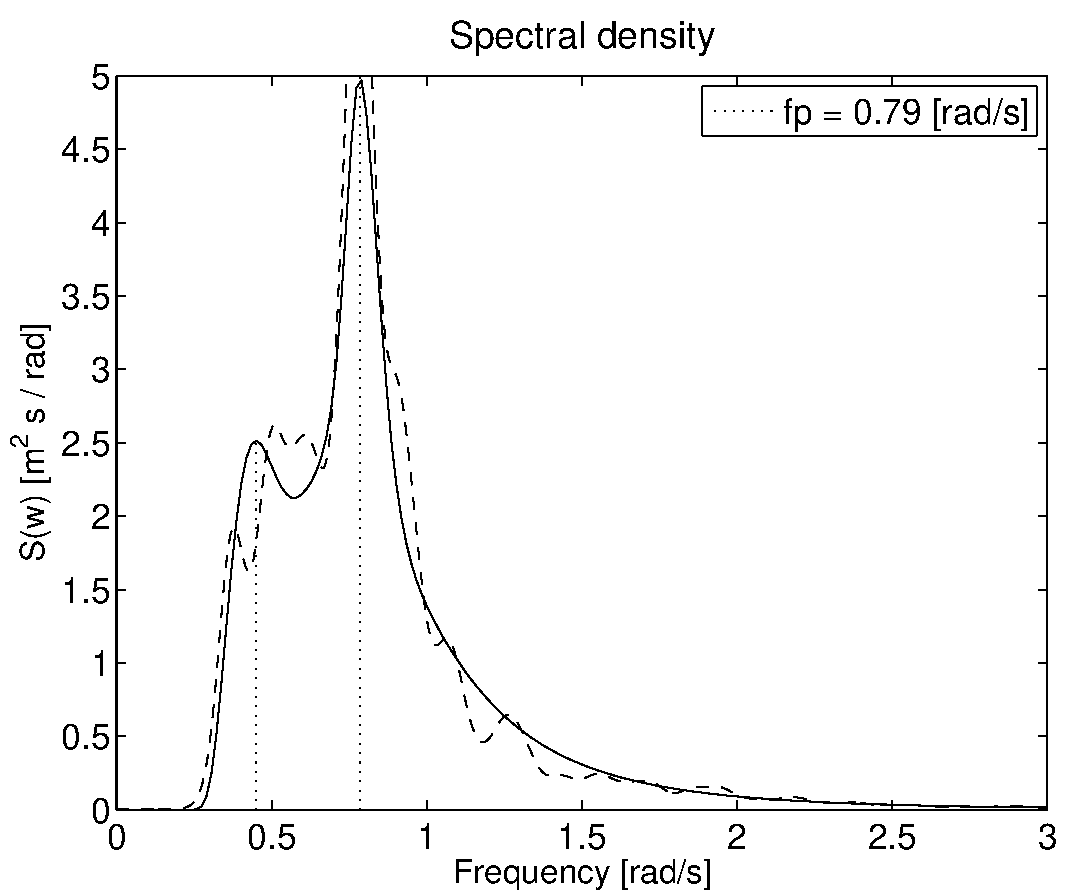
\includegraphics[width=\narrowfigwidth]{002f_spc}
\vspace{-3mm}
    \caption[Example of estimated spectrum]{Solid: 
      Thorsethaugen spectrum {\tt ST}.
  Dashed:  spectrum {\tt STest} estimated from
  data (20 minutes). % and 95\% confidence interval (dotted).
  Maximum lag size of Parzen window $=400$.}
  \label{fig:spectra}
  \end{figure}
  %-----
\label{page:torsethaugen}
  %-----
  %==============================================
  \subsection{Probability distributions of wave characteristics} %---
  %==============================================
  \progname{} gives the possibility to compute exact probability
  distributions for a number of wave characteristics, given a spectral
  density. A wave characteristic as, for example, wave period, can be
  defined in several ways, see Table~\ref{tab3_1}, page~\pageref{tab3_1}, in
  Chapter~\ref{cha:3}, and \progname{} allows the user to choose between
  a number of definitions: trough-to-crest, down-to-up crossing,
  up-to-up crossing, etc. In Chapter~\ref{cha:3} we analyse wave
  characteristics from observed data, and present some commonly used
  approximative distributions. Chapter~\ref{cha:4} describes how to use
  \progname{} to compute the exact theoretical distributions for
  all these wave characteristics in a
  Gaussian or transformed Gaussian model.

  In the numerical example, we consider the trough
  period, i.e.\ the down-to-up crossing definition. The wave periods
  can be extracted from the realization in Figure~\ref{fig:simulation}, and
  are shown as a histogram in Figure~\ref{fig:pdf}. This histogram may be
  compared to the theoretical density, calculated from the original
  spectrum $S(\omega)$, and from
  the estimated spectrum $S_{\mbox{\footnotesize est}}(\omega)$; see
  Figure~\ref{fig:pdf}. Recall that, for this spectrum,  $T_p=8$~[s].
  The figure shows the density for the half period; the
  results are in good agreement with that from the original spectrum. The
  following code lines are used to produced the presented figure. The
  different steps are: first extract half periods from the data by
  means of the routine \verb+dat2wa+ \index[xcmds]{{\tt dat2wa}}
  and store in the variable
  \verb+T+, then use \verb+spec2tpdf+ \index[xcmds]{{\tt spec2tpdf}}
  to calculate the theoretical
  distribution.
The parameter \verb+NIT+ determines the accuracy of the calculation.
  {\small\begin{verbatim}
        NIT = 3; paramt = [0 10 51]; clf
        dtyex = spec2tpdf(ST,[],'Tt',paramt,0,NIT);
        dtyest = spec2tpdf(STest,[],'Tt',paramt,0,NIT);
        [T, index] = dat2wa(xs,0,'d2u');
        histgrm(T,25,1,1), hold on
        pdfplot(dtyex), pdfplot(dtyest,'-.')
        axis([0 10 0 0.35]), hold off
\end{verbatim}}

%-----
\begin{figure}[tbh]
\centering
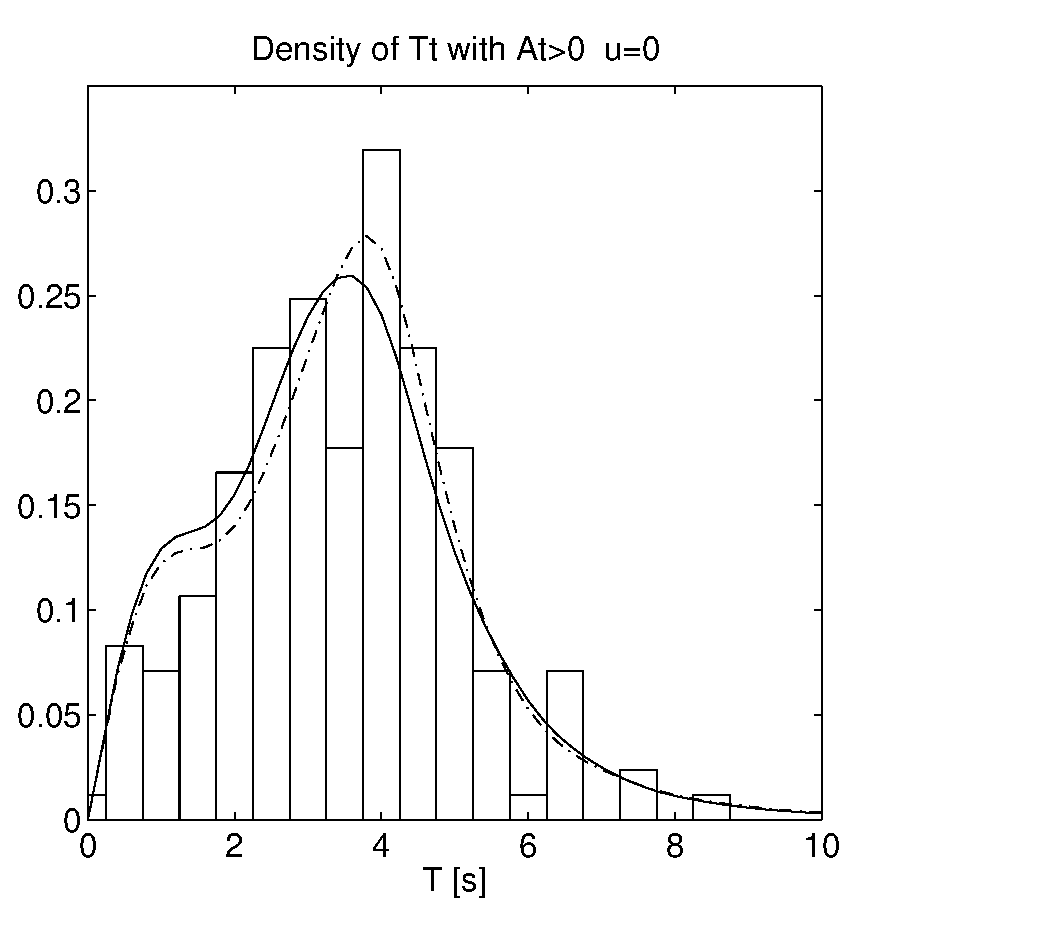
\includegraphics[width=\narrowfigwidth]{003f_pdf}
\vspace{-3mm}
\caption[Wave period, $T_{t}$, distribution]{
Pdf for wave  trough period for Torsethaugen spectrum {\tt ST} (solid line)
and estimated spectrum {\tt STest} (dash-dotted line).
The histogram shows the wave periods extracted from
the simulated data in Figure~\ref{fig:simulation}.}
\label{fig:pdf}
\end{figure}
%-----

%==============================================
\subsection{Directional spectra}\label{ss:dirspec}\index[xentr]{directional spectra}
\index[xentr]{spectrum!directional}
%==================
In \progname{} one finds means for evaluation and visualization of
directional spectra to model sea states with
waves coming from many different directions, that is
\[
   S(\omega,\theta)=S(\omega)\, D(\theta,\omega), \]
where $S(\omega)$ is a
frequency spectrum and $D(\theta,\omega)$ is a spreading function. A
number of common spreading functions can be chosen by the user.

One way of visualizing $S(\omega,\theta)$ is a polar plot. In
Figure~\ref{fig:directspect} we show the resulting directional spectrum
(solid line) for the Torsethaugen
spectrum  \index[xentr]{Torsethaugen!spectrum}
used above. The spreading \index[xentr]{spectrum!Torsethaugen}
function is of the \emph{cos-2s} type, that is (in the frequency
independent case),
\[
   D(\theta)=\frac{\Gamma(s+1)}{2\sqrt{\pi}\Gamma(s+1/2)}\cos^{2s}
    \left( \frac{\theta}{2} \right) \]
with $s\!\!=\!\!15$. Note that
the two peaks can be dis\-tinguished. The dash dotted line is the
corresponding result when the spreading function is frequency
dependent, cf.~\cite{KrogstadAndBarstow1999Directional}.
%Krogstad and Barstow (1999).

\begin{remark}``Wave direction''  is the direction from which waves are coming. 
\index[xentr]{wave!direction}
In \wf{} we adhere to the mathematical convention to count direction counter-clockwise 
from the positive $x$-axis. Thus, waves with direction 0$^o$ are coming from the East and 
waves with direction 90$^o$ are coming from the North, just the opposite to ocean standard. 
\end{remark}

Here are a few lines of code, which produce the graph of these
directional spectra with frequency independent and frequency dependent
spreading. The main directions are 90$^o$ and 0$^o$, respectively.
{\small\begin{verbatim}
    plotflag = 1; clf
    Nt = 101;   % number of angles
    th0 = pi/2; % primary direction of waves
    Sp = 15;    % spreading parameter
    D1 = spreading(Nt,'cos',th0,Sp,[],0); %frequency independent
    D12 = spreading(Nt,'cos',0,Sp,ST.w,1); %frequency dependent
    STD1 = mkdspec(ST,D1);  STD12 = mkdspec(ST,D12);
    plotspec(STD1,plotflag), hold on
    plotspec(STD12,plotflag,'-.'), hold off
\end{verbatim}}\index[xcmds]{{\tt mkdspec}}\index[xcmds]{{\tt plotspec}}

%-----
\begin{figure}[tbh]
  \centering
  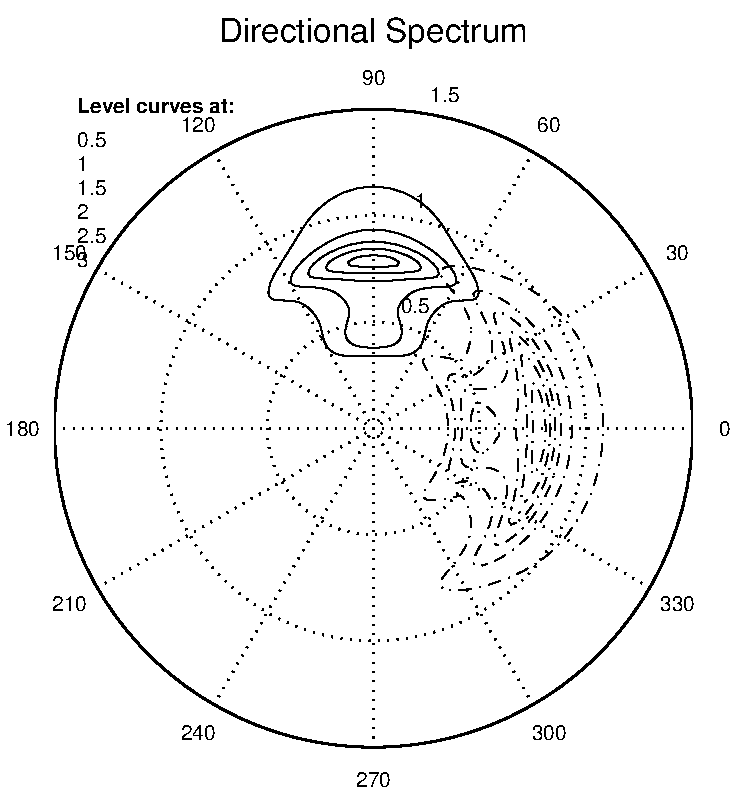
\includegraphics[width=\narrowfigwidth]{004f_drs}
\vspace{-3mm}
  \caption[Example of directional spectrum]{Directional spectrum.
  The frequency spectrum is a
  Torsethaugen spectrum and the spreading function is of \emph{cos-2s}
  type with $s = 15$. Solid line: directional spectrum with frequency
  independent spreading. Dash dotted line:
  directional spectrum, using frequency dependent spreading function.}
  \label{fig:directspect}
  \end{figure}
 %------

We finish the section with 20 seconds of simulated sea surfaces on 512[m] by 1024[m]
for a sea with directional spectra {\tt STD1} and {\tt STD12}. The
routine \verb+spec2field+ is used for simulation and the parameters 
for the simulation in space and time \index[xcmds]{{\tt simoptset}} 
are defined by the options function \verb+simoptset+. 
{\small\begin{verbatim}
    rng('default'); clf
    opt = simoptset('Nt',20,'dt',1,'Nu',1024','du',1,'Nv',512,'dv',1)
    W1 = spec2field(STD1,opt);
    W12 = spec2field(STD12,opt)
    
    W12 = struct with fields:
    Z: [512 x 1024 x 20 double]
    y: [1024 x 1 double]
    x: [512 x 1 double]
    t: [20 x 1 double]
\end{verbatim}}
\noindent
\index[xentr]{simulation!of sea surface}
\index[xcmds]{{\tt spec2field}}\index[xcmds]{{\tt simoptset}}
\index[xcmds]{{\tt seamovie}}

The generated space-time fields can be presented and optionally 
saved as a movie by the routine \verb+seamovie+. 
Specifying a file name saves the movie in avi-format, as for {\tt Movie12}.  
{\small\begin{verbatim}
    figure(1); clf
    Movie1 = seamovie(W1,1);
    figure(2); clf
    Movie12 = seamovie(W12,1,'GaussianSea12.avi')
\end{verbatim}

The last frame of the movies are shown in 
Figures~\ref{fig:00sima}-\ref{fig:00simb} and one can see that
waves are coming from different directions. However,
frequency dependent spreading leads to a more irregular
surface, so the orientation of waves is less transparent.
From the figures it is not easy to deduce that
both sea surfaces have the same period distribution, but
it is more obvious that the wavelength distributions are different.

\begin{figure}
  \centerline{
%\resizebox{\defwidth}{!}{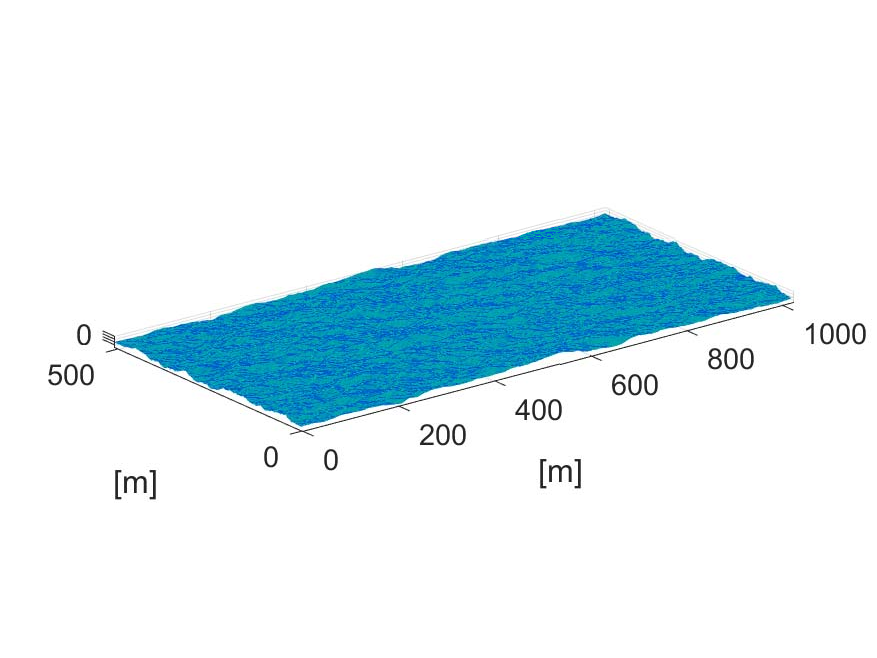
\includegraphics{fig_hav1aaa}}
\resizebox{0.95\textwidth}{!}{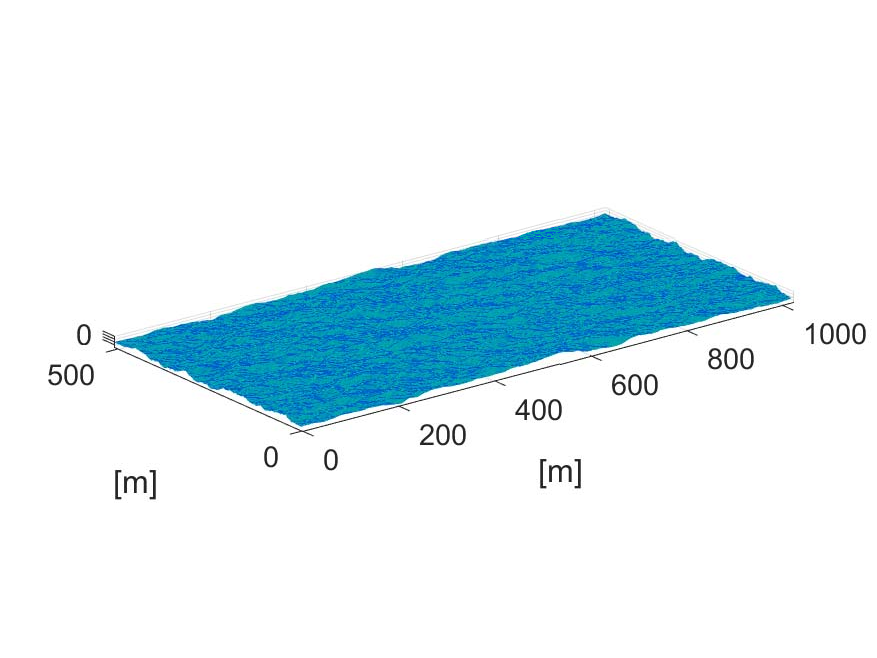
\includegraphics{fig_hav1aaa}}}
\vspace{-3mm}
\caption[Gaussian sea surface, frequency independent spreading]{Gaussian 
sea surface, 512 [m] by 1024 [m], with 
directional spectrum {\tt SD1}, spreading independent of frequency, waves from North.}
\label{fig:00sima}
\end{figure}
\begin{figure}
\centerline{
\resizebox{0.95\textwidth}{!}{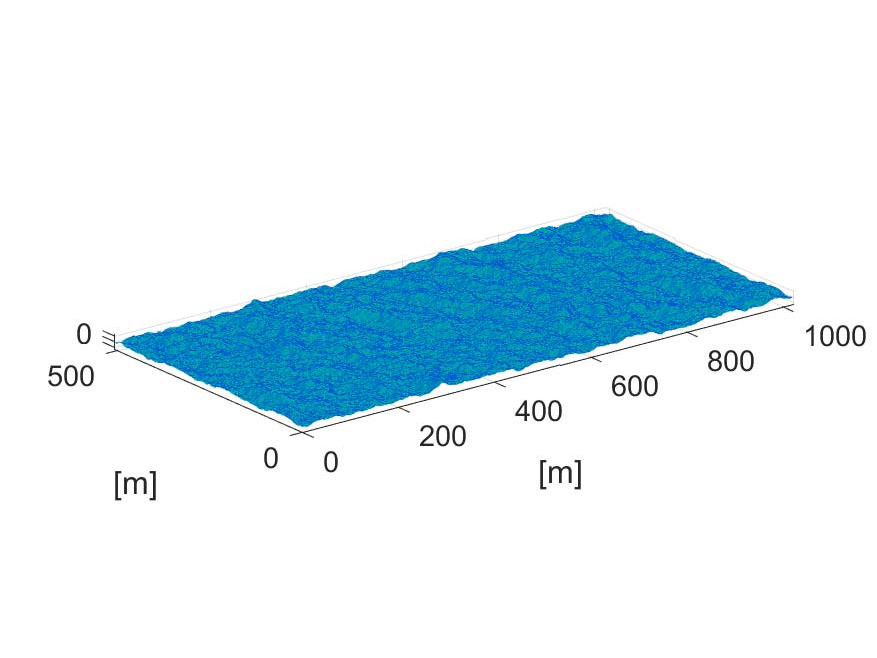
\includegraphics{fig_hav2aaa}}
}
\vspace{-3mm}
\caption[Gaussian sea surface, frequency dependent spreading]{Gaussian 
sea surface, 512 [m] by 1024 [m], with 
directional spectrum {\tt SD12}, frequency dependent spreading, waves from East.}
\label{fig:00simb}
\end{figure}

%==============================================
\subsection{Fatigue, load cycles, and Markov models}%---
%==============================================
In fatigue applications the exact sample path is not important, but
only the peaks and troughs of the load, called the  turning
points (TP). From these one can extract load cycles, from
which damage calculations and fatigue life predictions can be
performed. In \progname{}
there are numerous routines for evaluating fatigue measured loads, as
well as making theoretical calculations of distributions that are
important for fatigue evaluation.  A powerful technique when
analysing loads is to use Markov models as approximations, especially
to model the sequence of turning points by a Markov chain. For such
models there
exist many explicit results. Here, we will use this Markov
approximation for computing the intensity of rainflow cycles and
trough-to-crest cycles for the Gaussian model with spectrum from
Figure~\ref{fig:spectra}.

For fatigue analysis the rainflow cycle, defined in
Figure~\ref{FigRFCdef} in Chapter~\ref{cha:5}, is often used.
The Markov model is defined by the min-to-max pdf, which is obtained
from the power spectral density by using approximations in Slepian
model processes, see e.g.\
\cite{LindgrenAndRychlik1991Slepian} %LiRy91} %Lindgren and Rychlik~(1991)
and references therein. Chapter~\ref{cha:4} describes how \progname{}
routines can be used to find the min-to-max distribution for Gaussian loads.
For the Markov model, there is an explicit
solution for the intensity of rainflow cycles, see
\cite{FrendahlAndRychlik1993Rainflow}. \index[xentr]{min-to-max!pdf}
%,FrRy93}. %Frendahl and Rychlik~(1993).
By using the routines in \progname{} the intensity of rainflow cycles can be
found using Markov approximation; see Figure~\ref{fig:rainflow2}, where
also the rainflow cycles found in the simulated load signal are
shown. The figure has been plotted using the following commands:
{\small\begin{verbatim}
    paramu = [-6 6 61];
    frfc = spec2cmat(ST,[],'rfc',[],paramu);
    pdfplot(frfc); hold on
    tp = dat2tp(xs);      rfc = tp2rfc(tp);
    plot(rfc(:,2),rfc(:,1),'.'); hold off
\end{verbatim}}\index[xcmds]{{\tt spec2cmat}}
    \index[xcmds]{{\tt dat2tp}}\index[xcmds]{{\tt tp2rfc}}

%----- Figure
%-----
  \begin{figure}[tbh]
\centering
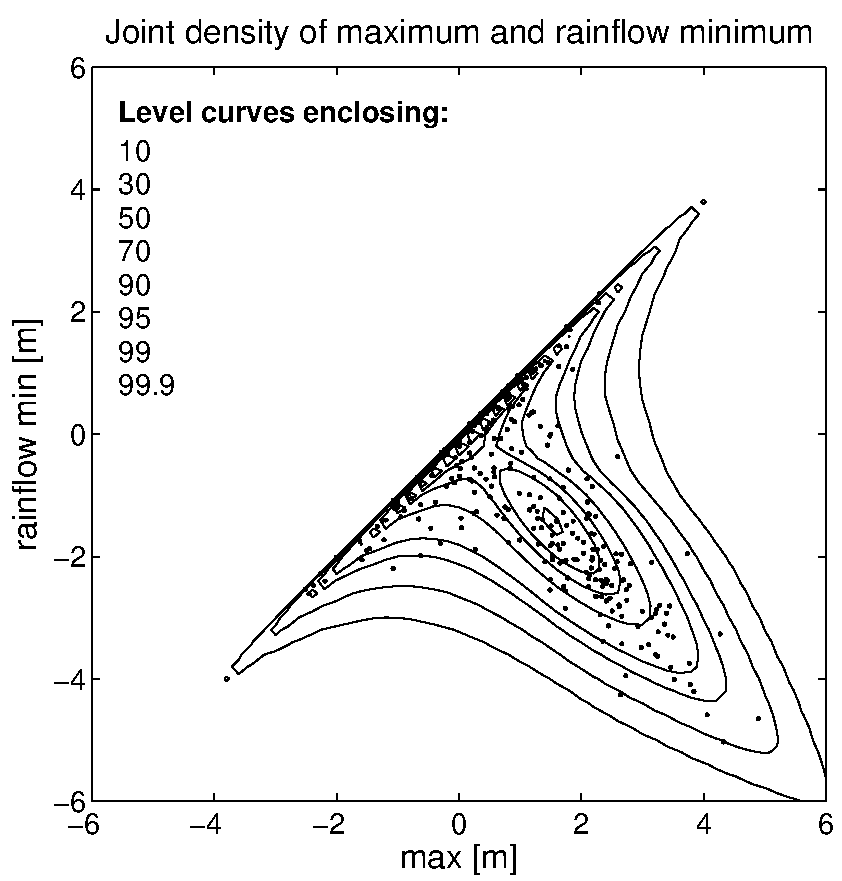
\includegraphics[width=\narrowfigwidth]{006f_rfc}
\vspace{-3mm}
\caption[Intensity of rainflow cycles]{Intensity of rainflow cycles
computed from the power spectrum through
  Markov approximation, compared with cycles found in the
  simulation. }
\label{fig:rainflow2}
\end{figure}
  %-----
  %----- End Figure

  \noindent
  The \progname{} toolbox also contains routines for computing the intensity
  of rainflow cycles in more complex load processes, for example
  for a switching Markov chain of turning points, {\tt TP}. Details on fatigue load analysis
are given in Chapter~\ref{cha:5}.

%==============================================
\subsection{Statistical extreme value analysis}\label{sec:extreme_example} %---
%==============================================
The {\sc Wafo}-toolbox contains almost 600 routines for general
statistical analysis, description, plotting, and simulation.
In Chapter~\ref{cha:6} we describe some routines which are particularly
important for wave and fatigue analysis, related to statistics of extremes.
These are based on the generalized extreme value (GEV) and generalized Pareto
distribution (GPD), combined with the peaks over threshold (POT) method.
\index[xentr]{Generalized Extreme Value!distribution, GEV}
\index[xentr]{Generalized Pareto!distribution, GPD}
As an example we show an analysis of wave elevation data from the
Poseidon platform in the Japan Sea. Data from about 23 hours of registration
are stored in the data set {\tt yura87}, taken with a 1~Hz sampling rate.
We first load and plot, in Figure~\ref{fig:yura87},
part of the data and calculate the maximum over 5 minute periods.
{\small\begin{verbatim}
      xn = load('yura87.dat'); subplot(211);
      plot(xn(1:30:end,1)/3600,xn(1:30:end,2),'.')
      title('Water level'), ylabel('m')
      yura = xn(1:85500,2);
      yura = reshape(yura,300,285);
      maxyura = max(yura); subplot(212)
      plot(xn(300:300:85500,1)/3600,maxyura,'.')
      xlabel('Time (h)'), ylabel('m')
      title('Maximum 5 min water level')
\end{verbatim}}

%----- Figure
%-----
  \begin{figure}[tbh]
\centering
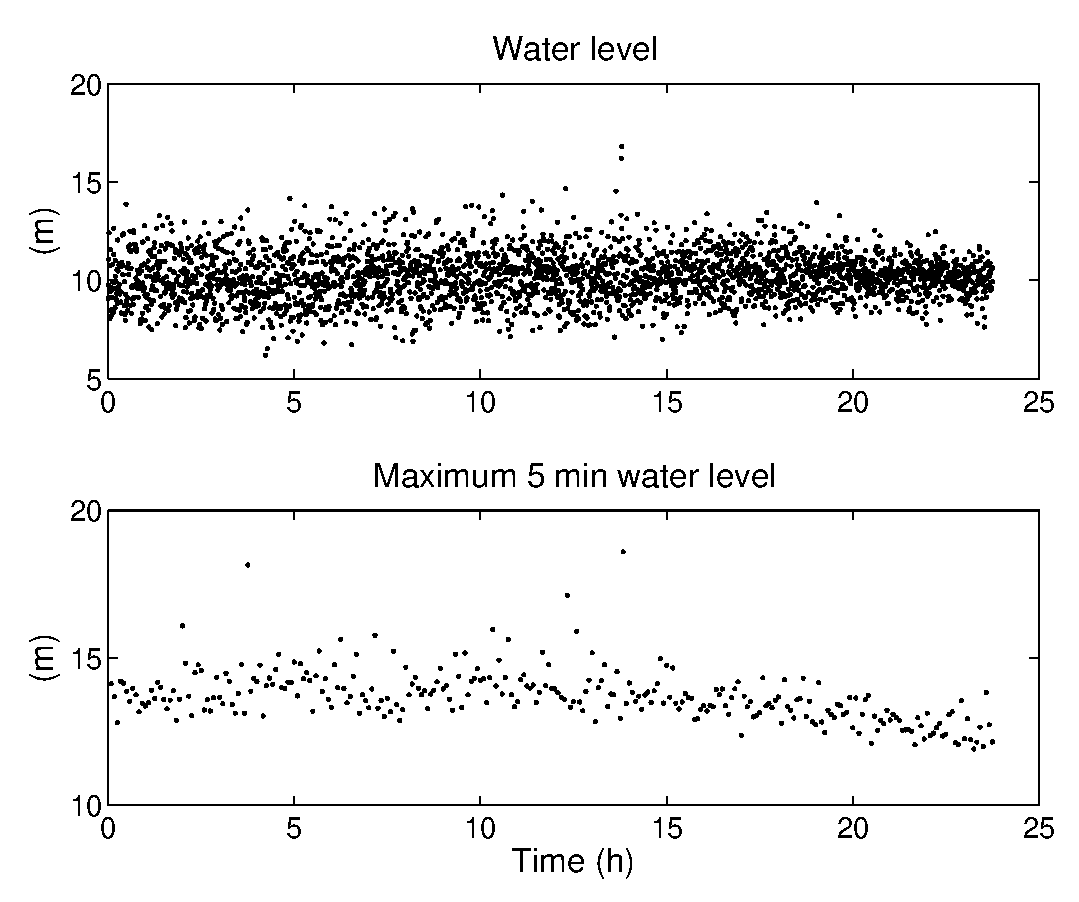
\includegraphics[width=0.85\textwidth]{007f_yura}
\vspace{-3mm}
\caption[Water level in the Japan Sea]{Water level variation in the Japan Sea
from the data set {\tt yura87} and maxima over 5~minute periods.}
\label{fig:yura87}
\end{figure}
  %-----
  %----- End Figure

\begin{figure}[tbh]
\centering
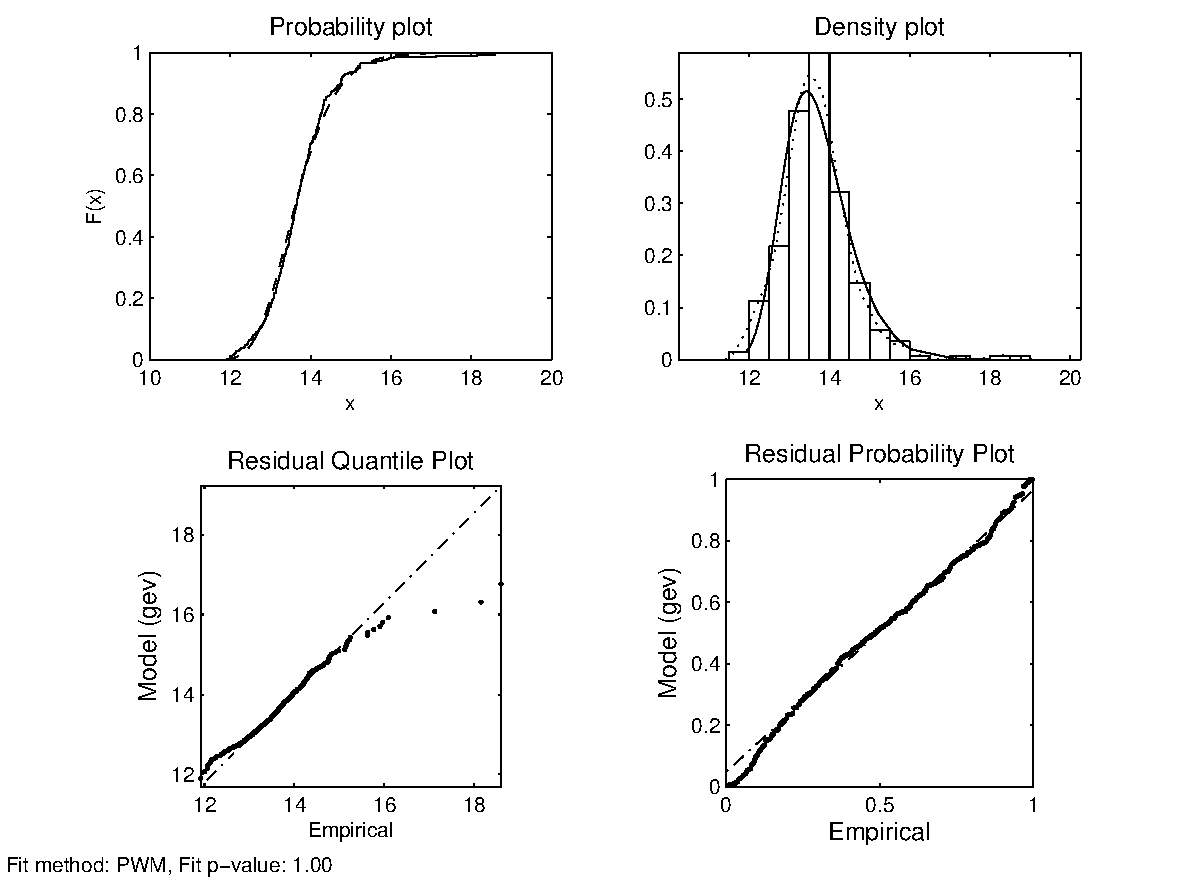
\includegraphics[width=0.85\textwidth]{008f_yuragev}
%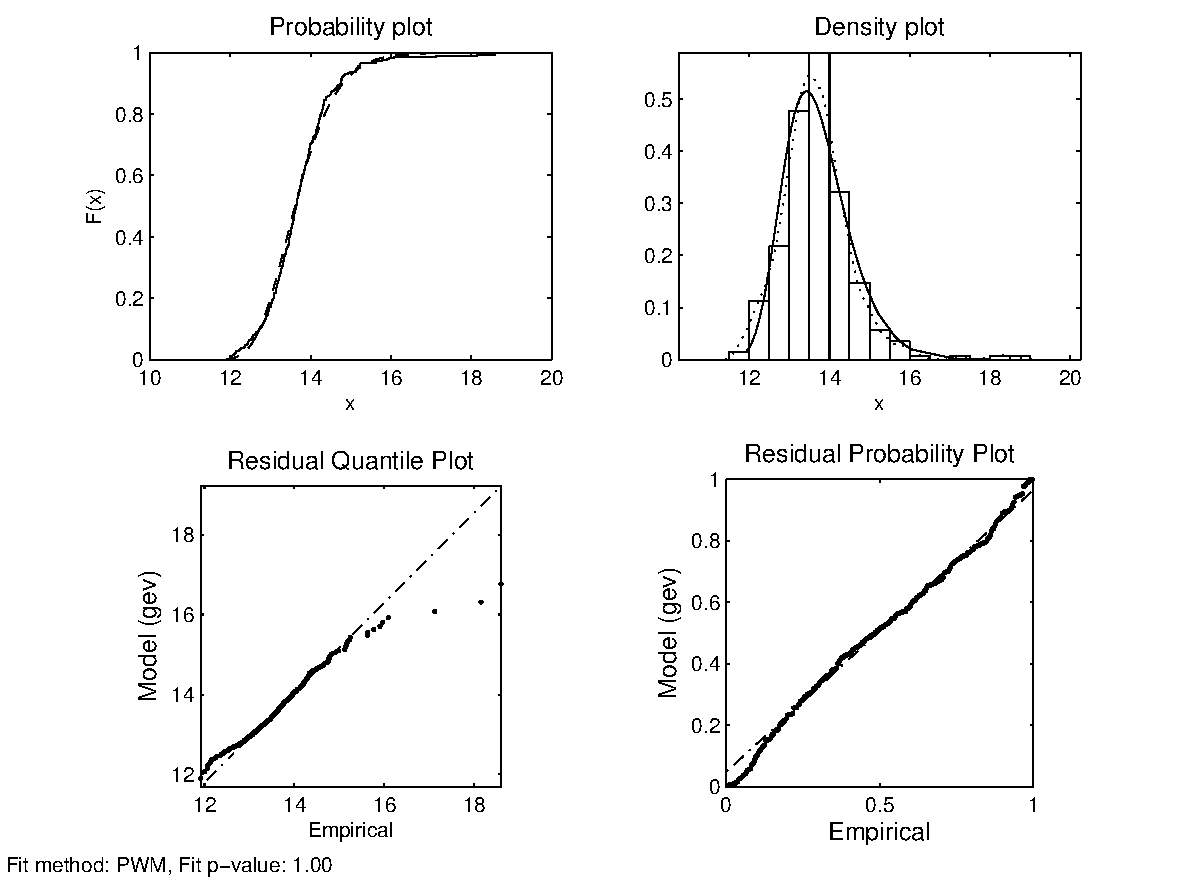
\includegraphics[width=100mm]{008f_yuragev}
\vspace{-3mm}
\caption[Extreme value analysis of {\tt yura87}]
{Diagnostic plots of GEV extreme value analysis of {\tt yura87}.}
\label{fig:yuragev}
\end{figure}

It is clear from the figures that there is a trend in the data, with
decreasing spreading with time. In Chapter~\ref{cha:5} we will deal with
that problem; here we make a crude extreme value analysis, by fitting a
GEV distribution to the sequence of 5 minute maxima,
simply by issuing the commands
{\small \begin{verbatim}
      phat = fitgev(maxyura,'plotflag',1);
\end{verbatim}}\index[xcmds]{{\tt fitgev}}
%This results in 

Figure~\ref{fig:yuragev}  shows cumulative distribution
and density of the fitted GEV distribution together with diagnostic
plots of empirical and model quantiles. The non-stationarity
gives a very bad fit in the upper tail of the distribution. The fitted GEV
has shape parameter $0.1$, with a 95\% confidence interval $(0.01, 0.18)$.
%\vspace{10mm}
%\newpage

%\clearpage
%\vspace{15cm}
%~

\section{Spectra used in the tutorial}\label{s:ListOfSpectra}
In this tutorial we illustrate the routines on many different wave and load spectra. 
Some are empirical, estimated from wave data, others are theoretical spectra 
suggested in the literature as suitable for special wave conditions. The following 
list and name convention 
should help the reader to keep track of the different types through the 
many examples in the next chapters.   The notation {\tt SXest} will occasionally be used 
for estimated spectra. 

\subsection{SG, Empirical spectrum from waves in {\tt gfaksr89.dat}}
Bi-modall spectrum {\tt SG} estimated at the Gullfaks~C platform at 2.5\:[Hz], 39\,000 data poins. 
This spectrum is used in Examples~\ref{Ex_preliminary_analysis}--\ref{Crest-trough-from-min-max}. 

\subsection{SJ, Theoretical {\sc Jonswap} spectrum}
Theoretical uni-modal {\sc Jonswap} spectrum {\tt SJ} designed for North Sea waves. 
This spectrum is used in Examples~\ref{Ex_sea_spectra}, \ref{Seamovieforexport}, and \ref{Ex_wave_parameters}.

\subsection{SS, Empirical spectrum from waves in {\tt sea.dat}}
Bi-modal spectrum {\tt SS}, estimated from shallow water wave data, 
sample rate 4\:[Hz], 9\,524 data points. This spectrum is used in Examples~\ref{Ex_sea_statistics}, 
\ref{Ex_sea_simulation}, \ref{rayleighapproximation}, \ref{Ex_Seadatawavedistributions}.

\subsection{ST, Theoretical {\sc Torsethaugen} spectrum}
Theoretical bi-modal {\sc Torsethaugen} spectrum {\tt ST} designed for mixed sea 
with wind waves and swell. This spectrum is used in Example~\ref{Ex_Torseth}.

% \subsection{SY, Empirical spectrum from waves in {\tt yura87.dat}}
%Uni-modal spectrum {\tt SY}, estimated from wave data, sample rate 1\:[Hz], 85\,547 data points.

\clearpage
%\newpage
\section{Datastructures}\label{sec:datastructures}
\index[xentr]{datastructures}\index[xentr]{structured array}
\vspace{-3mm}
{\small\begin{verbatim}
help datastructures

 DATASTRUCTURES of spectrum (S), covariance function (cvf)
 and probability density (pdf) in WAFO

  To represent spectra, covariance functions and probability
  density functions in WAFO, the MATLAB datatype 'structured
  array' is used. Here follows a list of the fields in
  the struct representing S, cvf and pdf, respectively.

  Spectrum structure
  ~~~~~~~~~~~~~~~~~~
   Requisite fields:
    .type  String: 'freq', 'dir', 'k2d', k1d', 'encdir', 'enc'.
    .S     Spectrum values (size=[nf 1] or [np nf]).
    .w OR .f OR .k Frequency/wave number lag, length nf.
    .tr    Transformation function (default [] (none)).
    .h     Water depth (default inf).
    .norm  Normalization flag, Logical 1 if S is normalized,
           0 if not.
    .note  Memorandum string.
    .date  Date and time of creation or change.
   Type-specific fields:
    .k2    Second dim. wave number lag,
           if .type='k2d', 'rotk2d', length np.
    .theta Angular lags, if .type='dir', 'rotdir' or 'encdir',
           length np.
    .v     Ship speed, if .type = 'enc' or 'encdir'.
    .phi   angle of rotation of the coordinate system
           (counter-clockwise) e.g. azimuth of a ship.

  See also  createspec, plotspec

  Covariance function (cvf) structure
  ~~~~~~~~~~~~~~~~~~~~~~~~~~~~~~~~~~~
    .R     Covariance function values, size [ny nx nt],
           all singleton dim. removed.
    .x     Lag of first space dimension, length nx.
    .y     Lag of second space dimension, length ny.
    .t     Time lag, length nt.
    .h     Water depth.
    .tr    Transformation function.
    .type  'enc', 'rot' or 'none'.
    .v     Ship speed, if .type='enc' .
    .phi   Rotation of coordinate system, e.g. direction of ship.
    .norm  Normalization flag, Logical 1 if autocorrelation,
           0 if covariance.
    .Rx ... .Rtttt   Obvious derivatives of .R.
    .note  Memorandum string.
    .date  Date and time of creation or change.

  See also  createcov, spec2cov, cov2spec, covplot

  Probability density function (pdf) structure
  ~~~~~~~~~~~~~~~~~~~~~~~~~~~~~~~~~~~~~~~~~~~~
  Describing a density of n variables:
    .f     Probability density function values,
           (n-dimensional matrix).
    .x     Cell array of vectors defining grid for variables,
           (n cells).
    .labx  Cell array of label strings for the variables,
           (n cells).
    .title Title string.
    .note  Memorandum string.

  See also  createpdf, pdfplot
\end{verbatim}
}

%\bibliography{wafoBibliography}

%%% Local Variables:
%%% mode: latex
%%% TeX-master: "wafomanual"
%%% End:
